\documentclass[12pt]{jbook}
% shuron.sty �δ��������ɤ�����
\usepackage{fancyhd,shuron}
\usepackage{graphics}
\usepackage[dvipdfmx]{graphicx}
\usepackage{epsfig}
\usepackage{tabularx}
\usepackage{chapterbib}
\usepackage{makeidx}
\usepackage{amssymb}
\usepackage{url}
\usepackage{slashbox}
% �ɲ�
\usepackage{booktabs}

\makeatletter
\def\thefootnote{\ifnum\c@footnote>\z@\leavevmode\lower.5ex%
    \hbox{$^{*\@arabic\c@footnote}$}\fi}
\makeatother

\makeindex

% http://www.lab2.kuis.kyoto-u.ac.jp/~okita/etc/#0011
%%% jdummy.def
%
\DeclareRelationFont{JY1}{mc}{it}{}{OT1}{cmr}{it}{}
\DeclareRelationFont{JT1}{mc}{it}{}{OT1}{cmr}{it}{}
\DeclareFontShape{JY1}{mc}{m}{it}{<5> <6> <7> <8> <9> <10> sgen*min
    <10.95><12><14.4><17.28><20.74><24.88> min10
    <-> min10}{}
\DeclareFontShape{JT1}{mc}{m}{it}{<5> <6> <7> <8> <9> <10> sgen*tmin
    <10.95><12><14.4><17.28><20.74><24.88> tmin10
    <-> tmin10}{}
\DeclareRelationFont{JY1}{mc}{sl}{}{OT1}{cmr}{sl}{}
\DeclareRelationFont{JT1}{mc}{sl}{}{OT1}{cmr}{sl}{}
\DeclareFontShape{JY1}{mc}{m}{sl}{<5> <6> <7> <8> <9> <10> sgen*min
    <10.95><12><14.4><17.28><20.74><24.88> min10
    <-> min10}{}
\DeclareFontShape{JT1}{mc}{m}{sl}{<5> <6> <7> <8> <9> <10> sgen*tmin
    <10.95><12><14.4><17.28><20.74><24.88> tmin10
    <-> tmin10}{}
\DeclareRelationFont{JY1}{mc}{sc}{}{OT1}{cmr}{sc}{}
\DeclareRelationFont{JT1}{mc}{sc}{}{OT1}{cmr}{sc}{}
\DeclareFontShape{JY1}{mc}{m}{sc}{<5> <6> <7> <8> <9> <10> sgen*min
    <10.95><12><14.4><17.28><20.74><24.88> min10
    <-> min10}{}
\DeclareFontShape{JT1}{mc}{m}{sc}{<5> <6> <7> <8> <9> <10> sgen*tmin
    <10.95><12><14.4><17.28><20.74><24.88> tmin10
    <-> tmin10}{}
\DeclareRelationFont{JY1}{gt}{it}{}{OT1}{cmbx}{it}{}
\DeclareRelationFont{JT1}{gt}{it}{}{OT1}{cmbx}{it}{}
\DeclareFontShape{JY1}{mc}{bx}{it}{<5> <6> <7> <8> <9> <10> sgen*goth
    <10.95><12><14.4><17.28><20.74><24.88> goth10
    <-> goth10}{}
\DeclareFontShape{JT1}{mc}{bx}{it}{<5> <6> <7> <8> <9> <10> sgen*tgoth
    <10.95><12><14.4><17.28><20.74><24.88> tgoth10
    <-> tgoth10}{}
\DeclareRelationFont{JY1}{gt}{sl}{}{OT1}{cmbx}{sl}{}
\DeclareRelationFont{JT1}{gt}{sl}{}{OT1}{cmbx}{sl}{}
\DeclareFontShape{JY1}{mc}{bx}{sl}{<5> <6> <7> <8> <9> <10> sgen*goth
    <10.95><12><14.4><17.28><20.74><24.88> goth10
    <-> goth10}{}
\DeclareFontShape{JT1}{mc}{bx}{sl}{<5> <6> <7> <8> <9> <10> sgen*tgoth
    <10.95><12><14.4><17.28><20.74><24.88> tgoth10
    <-> tgoth10}{}
\DeclareRelationFont{JY1}{gt}{sc}{}{OT1}{cmbx}{sc}{}
\DeclareRelationFont{JT1}{gt}{sc}{}{OT1}{cmbx}{sc}{}
\DeclareFontShape{JY1}{mc}{bx}{sc}{<5> <6> <7> <8> <9> <10> sgen*goth
    <10.95><12><14.4><17.28><20.74><24.88> goth10
    <-> goth10}{}
\DeclareFontShape{JT1}{mc}{bx}{sc}{<5> <6> <7> <8> <9> <10> sgen*tgoth
    <10.95><12><14.4><17.28><20.74><24.88> tgoth10
    <-> tgoth10}{}
\DeclareRelationFont{JY1}{gt}{it}{}{OT1}{cmr}{it}{}
\DeclareRelationFont{JT1}{gt}{it}{}{OT1}{cmr}{it}{}
\DeclareFontShape{JY1}{gt}{m}{it}{<5> <6> <7> <8> <9> <10> sgen*goth
    <10.95><12><14.4><17.28><20.74><24.88> goth10
    <-> goth10}{}
\DeclareFontShape{JT1}{gt}{m}{it}{<5> <6> <7> <8> <9> <10> sgen*tgoth
    <10.95><12><14.4><17.28><20.74><24.88> tgoth10
    <-> tgoth10}{}
\endinput
%%%% end of jdummy.def


\begin{document}
\setcounter{page}{0}
\thispagestyle{empty}

\noindent

\includegraphics[height=2.0cm]{img/Lissajous_UEC_logo.eps}\\
\begin{tabular}{c}
{\Large ʿ��XXǯ�� ������ʸ}				\\
\end{tabular}

\vspace{2.5cm}

\begin{center}
\LARGE \bf ���������ȥ�\\
%\vspace{4mm}
\end{center}

\vspace{1.5cm} 

\LARGE
\begin{flushright}
�ŵ��̿���� ��ر� ���������\\
�ߡ��칶\\
1234567  ̾��\\

\vspace{1.6zh}

{\def\arraystretch{0.6}
\begin{tabular}{rll@{}}
��Ƴ����	& ���� ����& ����	\\
		& ���� ����& ����	\\
		& ���� ����& ����\\
							\\
�����	& \multicolumn{2}{c@{}}{ʿ��XXǯ1��30��}	\\
\end{tabular}
}
\end{flushright}
\normalsize
\newpage

\thispagestyle{empty}

\noindent
\begin{center}
\LARGE \bf ����\\
\end{center}

\vspace{1.0cm} 
{\small
����(���֥��ȥ饯��)�ϾϤȤ������ʲ������Ƥ�1�ڡ����������ɤ��ޤȤ�롥

\begin{itemize}
\setlength{\itemsep}{-2mm}
\item ������ط�(�ؽ�Ū���Ҳ�Ū)
\item ��Ū
\item ��ˡ
\item ����
\end{itemize}

���������� ���������� ���������� �����ĤƤ�
���������� ���������� ���������� �����ĤƤ�
���������� ���������� ���������� �����ĤƤ�
���������� ���������� ���������� �����ĤƤ�
���������� ���������� ���������� �����ĤƤ�
���������� ���������� ���������� �����ĤƤ�
���������� ���������� ���������� �����ĤƤ�
���������� ���������� ���������� �����ĤƤ�

�ʤˤ̤ͤ� �ϤҤդؤۡ��ޤߤ��� �䤤�椨��
�ʤˤ̤ͤ� �ϤҤդؤۡ��ޤߤ��� �䤤�椨��
�ʤˤ̤ͤ� �ϤҤդؤۡ��ޤߤ��� �䤤�椨��
�ʤˤ̤ͤ� �ϤҤդؤۡ��ޤߤ��� �䤤�椨��
�ʤˤ̤ͤ� �ϤҤդؤۡ��ޤߤ��� �䤤�椨��
�ʤˤ̤ͤ� �ϤҤդؤۡ��ޤߤ��� �䤤�椨��
�ʤˤ̤ͤ� �ϤҤդؤۡ��ޤߤ��� �䤤�椨��
�ʤˤ̤ͤ� �ϤҤդؤۡ��ޤߤ��� �䤤�椨��
�ʤˤ̤ͤ� �ϤҤդؤۡ��ޤߤ��� �䤤�椨��
�ʤˤ̤ͤ� �ϤҤդؤۡ��ޤߤ��� �䤤�椨��

���� ���� ���� ���� ���� ���� ����
���� ���� ���� ���� ���� ���� ����
���� ���� ���� ���� ���� ���� ����
���� ���� ���� ���� ���� ���� ����
���� ���� ���� ���� ���� ���� ����
���� ���� ���� ���� ���� ���� ����

�ʡ������Ԥä���
}
\normalsize
\newpage


\setcounter{page}{1}

% �ܼ�
\tableofcontents
% ���ܼ�
\listoffigures
% ɽ�ܼ�
\listoftables

% ��ʸ����
%���_�w�i�ƖړI
\chapter{����}\label{chap:introduction}

\section{�ط�}
���󥿡��ͥåȤ򰭻������Ѥ����ڤϸ���ɤ��������ޤ��ޤ������ĤĤ��롥
���ϡ����ޤ��ޤʼ�ˡ�ǰ�����Ԥ��ĤĤ��뤿�ᡤ������Ф����к���Ƥ����
�ͥåȥ���������ƥ��ν������������ĤĤ���\cite{ipsj-thesisformat}��
������桤

\section{�ܸ������Ū}

�ܸ������Ū�ϡ���
�ܸ������Ū�ϡ�������������
�ܸ������Ū�ϡ���������������������������������
�ܸ������Ū�ϡ���������������������������������
�ܸ������Ū�ϡ���������������������������������
�ܸ������Ū�ϡ���������������������������������
�ܸ������Ū�ϡ���������������������������������
�ܸ������Ū�ϡ���������������������������������
�ܸ������Ū�ϡ���������������������������������
�ܸ������Ū�ϡ���������������������������������
�ܸ������Ū�ϡ���������������������������������
�ܸ������Ū�ϡ���������������������������������
�ܸ������Ū�ϡ���������������������������������
�ܸ������Ū�ϡ���������������������������������
�ܸ������Ū�ϡ���������������������������������

\subsection{�ܸ���ο�����Ū}
\label{subsec:ura}

�ܸ���ο�����Ū�ϡ���������������������������������
�ܸ���ο�����Ū�ϡ��ܸ���ο�����Ū�ϡ�
�ܸ���ο�����Ū�ϡ��ܸ���ο�����Ū�ϡ��ܸ���ο�����Ū�ϡ�
�ܸ���ο�����Ū�ϡ��ܸ���ο�����Ū�ϡ��ܸ���ο�����Ū�ϡ��ܸ���ο�����Ū�ϡ�

\subsubsection{�ܸ����΢����Ū}

�����ͤ�\cite{Findlater:2011}
����⤤���ͤ�\cite{motomura:2000-11-15}
�����äȡ����줬���֤���\cite{ipsj-thesisformat}��
����Ϥ��ä����ܤ��̤��Ƥ������ȡ�

\url{http://www.google.com/} \\
\url{https://milano.az.inf.uec.ac.jp/~zetaka/labwiki/}

\newpage

\section{��ʸ�ι���}
����ʸ�ϰʲ��ξϤˤ�깽������롥\\

�� \ref{chap:introduction} �� �����Ǥϡ����˴ؤ����ä򤷡�\
�� \ref{chap:relatedwork} �� ��Ϣ����ξϤǤϡ����ϤǽҤ٤���������
�Ф����¸�����ʤ並��μ���Ȥߤ�Ҳ𤹤롥�ޤ�����ˤȤ�ʤ����ɤΤ褦��
��ˡ���к��Ȥ����Ѥ����Ƥ��뤫���������롥
�� \ref{chap:system} �� �����ƥ�Ǥϡ��ܸ���dz�ȯ���������ƥ�˴ؤ��븶���Ⱦܺ�������Ԥ����� \ref{chap:results} �� ��̤Ǥϡ��ʤ�餫�η�̤ˤĤ�����𤹤롥
�� \ref{chap:discussion} �� �ͻ��Ǥϡ�����ޤǤμ���Ȥߤ�����줿��̤��顤
�ܸ�������̤ȳƷ�̤��Ф���ͻ����ʤ�Ӥ˺���β���ˤĤ��ƹͻ����롥\\
�� \ref{chap:conclusion} �� �������ܸ���ˤĤ������礹�롥\\

\newpage


%�֘A����
\chapter{��Ϣ����}\label{chap:relatedwork}

����ʤ�Τ⤢��ޤä���
\ref{chap:introduction}�Ϥˤ�񤭤ޤ�������

\section{A�δ�Ϣ����}
\label{sec:relatedworkA}

\ref{subsec:ura}��ˡ��ܸ���ο�����Ū��񤤤�����������ͳ�Ϥ��δ�Ϣ����ˤ��롥

\newpage

%�V�X�e��
\chapter{�����ƥ�}\label{chap:system}

�ɤ��ʤΡ������ʤ�

\begin{figure}[th]
\begin{center}

\epsfig{file=img/Lissajous_UEC_logo.eps,scale=0.50}
\caption{�ꥵ������޷�}
\end{center}
\label{fig:lissajous}
\end{figure}


\newpage


%����
\chapter{���}\label{chap:results}

����ʤ��̤Ǥޤ������ɡ��ɤʤ��Ǥä������

\begin{figure}[ht]
\begin{center}
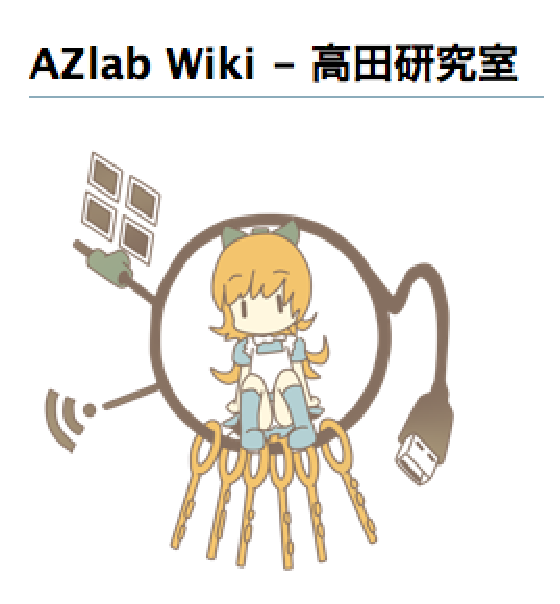
\includegraphics[scale=1.0]{img/azlabMark.eps}
\caption{our lab's web page}
\label{fig:azweb}
\end{center}
\end{figure}

��\ref{fig:azweb}�ϡ���ʬ����Υ���ܥ�ޡ���

\newpage


%�l�@
\chapter{�ͻ�}\label{chap:discussion}

\begin{table}[th]
	\begin{center}
		\caption{�ʤ�Τ����ɽ}
		\label{tbl:hyou}
		\vspace{4mm}
		\scalebox{1.0}{
			\begin{tabular}{ccc}
			\toprule
			���� & ���� & �褳 \\
			\midrule
			���� & 1cm & 2cm \\
			���� & 1.22cm & 2.87cm \\
			\bottomrule
			\end{tabular}
		}
	\end{center}
\end{table}

\begin{table}[th]
	\begin{center}
		\caption{������������ˡ}
		\vspace{4mm}
		\scalebox{1.0}{
			\begin{tabular}{ccc}
				\toprule
				\multicolumn{2}{c}{2��֤�} & 1��֤� \\
				\midrule
				a & f & k \\
				b & g & l \\
				c & h & m \\
				d & i & n \\
				e & j & o \\
				\bottomrule
			\end{tabular}
		}
	\end{center}
\end{table}

���������ͤ�����
���������������� ���������������� ���������������� ����������������
���������������� ���������������� ���������������� ����������������
���������������� ���������������� ���������������� ����������������
���������������� ���������������� ���������������� ����������������
���������������� ���������������� ���������������� ����������������
���������������� ���������������� ���������������� ����������������
���������������� ���������������� ���������������� ����������������
���������������� ���������������� ���������������� ����������������
���������������� ���������������� ���������������� ����������������
���������������� ���������������� ���������������� ����������������
���������������� ���������������� ���������������� ����������������
���������������� ���������������� ���������������� ����������������
���������������� ���������������� ���������������� ����������������
���������������� ���������������� ���������������� ����������������
���������������� ���������������� ���������������� ����������������
���������������� ����������������
���������������� ���������������� ���������������� ����������������
���������������� ���������������� ���������������� ����������������
���������������� ���������������� ���������������� ����������������

\newpage


%���_
\chapter{����}\label{chap:conclusion}

\newpage

%�ӎ�
\begin{ackn}{}

���դ��ޤ���
��塤��塤��²�Τߤ�ʡ�
���������漼�ν���������������Ʊ���Τߤ�ʡ�

\end{ackn}{}
\newpage
% LocalWords:  ackn

%�Q�l����
%\begin{thebibliography}{99}

<<<<<<< HEAD
% アルファベット順にソート
%\bibliographystyle{plain}
% 出現順にソート
\bibliographystyle{junsrt}
=======
%\bibliographystyle{plain}
\bibliographystyle{unsrt}
>>>>>>> f48b99123758dc1137e472207901c310cd4079a4
\bibliography{documents/bibtex}

\newpage

%\end{thebibliography}


% ��Ͽ
%\appendix
\chapter{��Ͽ}
\section{����ץ�ץ������Ǥ��Τ�} \label{app:sample_program}
ruby 1.9.2p290 (2011-07-09 revision 32553) x86 64-darwin10.8.0 �ˤ�ư����ǧ������
\lstinputlisting[language=Ruby]{programs/sample_program.rb}


%\addcontentsline{toc}{chapter}{����}
%\printindex

\end{document}
